%The Introduction section clarifies the motivation for the work presented and prepares readers for the structure of the paper.
% context:  orient those readers who are less familiar with your topic and to establish the importance of your work
% need: state the need for your work, as an opposition between what the scientific community currently has and what it wants.
% task: indicate what you have done in an effort to address the need (this is the task)
% object: preview the remainder of the paper to mentally prepare readers for its structure, in the object of the document
%%%%%%%%%%%%%%%%%%%%%%%%%%%%%%%%%%%%%%%%%%%%%%%%%%%%%%%%%%%%%%%%%%%%%%%%%%%%%%%
\section{Introduction}
\label{sec:Introduction}
%%%%%%%%%%%%%%%%%%%%%%%%%%%%%%%%%%%%%%%%%%%%%%%%%%%%%%%%%%%%%%%%%%%%%%%%%%%%%%%

The performance of these microscopes is often compromised by aberrations that lead to a reduction image resolution and contrast. 

These aberrations may arise from imperfections in the optical system or may be introduced by the physical properties of the specimen.
 
The problems caused by aberrations can be overcome using adaptive optics, whereby aberrations are corrected using a dynamic element, such as a deformable mirror.

This technology was originally conceived for the compensation of the aberrating effects of the atmosphere and was first developed for military and astronomical telescopes. 

Adaptive optics systems have also been introduced for other applications such as laser beam shaping, optical communications, data storage, ophthalmology and microscopy.\\
Hellooooooooo

\cite{Aberrations_book} 



For the purpose of understanding the operation of an adaptive optical system, it is best to think of aberrations in terms of distortions of an optical wavefront.

\begin{figure}[tbh]
        \centering
        \begin{subfigure}[b]{0.4\textwidth}
                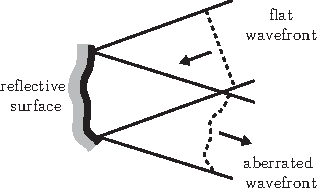
\includegraphics[width=\textwidth]{images/wavefront_distortions_reflection}
                \caption{Reflection.}
                \label{fig:abberation_reflection}
        \end{subfigure}
				\hspace{1em}
        \begin{subfigure}[b]{0.3\textwidth}
                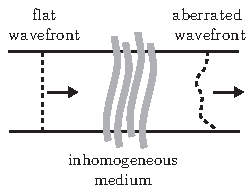
\includegraphics[width=\textwidth]{images/wavefront_distortions_transmission}
                \caption{Transmission.}
                \label{fig:abberation_trans}
        \end{subfigure}
        \caption{Wavefront aberrations due to (a) reflection from a non planar surface and (b)  caused by propagation through a non-uniform refractive index distribution. Image after~\cite{Aberrations_book}.}
\label{fig:abberations}
\end{figure} 

Representing aberrations in this way can simplify the design, control and characterisation of adaptive optics. The choice of modes for a particular application is often influenced by some aspect of the system, such as the deformation modes of a deformable mirror or the statistics of the induced aberrations. Otherwise, the modal representation may be chosen through mathematical convenience. For example, Zernike polynomials are often used for systems with circular apertures as they form a complete, orthogonal set of functions defined over a unit circle

\begin{figure}[htbp]
	\centering
		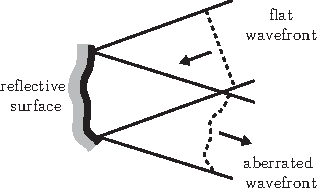
\includegraphics[width=0.30\textwidth]{images/wavefront_distortions_reflection.pdf}
	\caption{This is my first image.}
	\label{fig:wavefront_distortions_reflection}
\end{figure}

As with all optical systems, microscopes can also suffer from aberrations due to imperfections in the optical components. In practice, no system can be totally free from aberrations and so systems are designed to maintain aberrations below a particular tolerance for a given set of imaging conditions, such as wavelength, magnification and field of view. Significant aberrations can be introduced if a microscope is used outside its design specifications, for example at the incorrect wavelength or at a difierent temperature (see Chapter 11 of Ref. 9).